%============================================================================
%       CCM Tools - Tutorial
%
% $Id$
%=============================================================================

% PAKETE =====================================================================
\documentclass{report}

\usepackage{times}
\usepackage[T1]{fontenc}
\usepackage{a4}
\usepackage{graphicx}

% new float environment for example code, using framed verbatim minipages.
\usepackage{float}
\newfloat{Example}{htb}{loe}[section]

\setlength{\fboxsep}{5mm}
\newlength{\minifboxwidth}
\setlength{\minifboxwidth}{\columnwidth}
\addtolength{\minifboxwidth}{-5mm}
\newsavebox{\fmbox}
\newenvironment{minifbox}
  {\begin{lrbox}{\fmbox}\begin{minipage}{\minifboxwidth}}
  {\end{minipage}\end{lrbox}\fbox{\usebox{\fmbox}}}

% length definitions for paragraph spacing and indent.
\setlength{\parindent}{0cm}

% custom controls over float placement and page flow.
\renewcommand{\textfraction}{0.05}
\renewcommand{\topfraction}{0.95}
\renewcommand{\bottomfraction}{0.95}
\renewcommand{\floatpagefraction}{0.1}
\setcounter{totalnumber}{5}

%=Content======================================================================
\title{{\Huge CCM Tools}\\Tutorial}

\author{
  Egon Teiniker <egon.teiniker@tugraz.at>\\
  Leif Johnson <leif@ambient.2y.net>\\
%  \vspace{1em}
%  {\small $Id$}
}

\begin{document}
\maketitle
\pagenumbering{roman}
\tableofcontents
\listoffigures

\newpage
\pagenumbering{arabic}
\setlength{\parskip}{1em}

%******************************************************************************
\chapter{Introduction}
\label{chapter:introduction}
%******************************************************************************

The CCM Tools are a set of programs and libraries used to generate, package and
deploy CORBA components. The tools implement parts of the CCM specification
\cite{CCMSpecification} with some extensions to improve the usability and
performance of the component model. The {\it CCM Tools User's Guide\/} provides
instructions for using the CCM Tools. This document, the {\it CCM Tools
Developer's Manual\/}, is aimed at developers and provides details on the inner
workings of the CCM Tools.

\begin{figure}
\centering \includegraphics[width=14cm]{ToolsOverview}
\caption{Parts of the CCM Tools package.}
\label{fig:intro-ToolsOverview}
\end{figure}

To help the component developer, the CCM Tools provide the tools shown in
Figure~\ref{fig:intro-ToolsOverview}. These tools include the following parts:

\paragraph{CCM Metamodel Library}

The CCM specification defines a metamodel for the IDL3 syntax. This metamodel is
a set of classes that are capable of representing the syntactic elements in
IDL3. We implemented a metamodel library in Java that allows creation of, and
navigation through, CCM models. Using this library we can clearly separate the
parser and the code generators, using a CCM model as the communication between
the two parts. The parser creates a model object for every part of the source
code matching an IDL grammar rule, and the generator tools read the model to
generate code. Chapter~\cite{chapter:ccm-metamodel-library} describes the CCM
Tools' construction of the CCM metamodel library.

\paragraph{IDL3 Parser}

The IDL3 Parser reads an IDL3 file, checks the syntax of the IDL source code and
creates a CCM model, using the CCM metamodel library, in memory. This CCM model
is the starting point for all code generator tools.
Chapter~\cite{chapter:idl3-parser} describes the IDL3 parser in detail.

\paragraph{Mirror Component Generators}

After building a component it is a good idea to run a set of functional tests on
it. Such testing can provide helpful component specific debugging and prevent
large, difficult to locate, system bugs later in development.

To provide a test environment for every component, the CCM Tools can create a
mirror component (a facet becomes a receptacle and vice versa) described in a
mirror IDL3 file. We use the C++ component generators with the mirror IDL3 files
to generate the code for mirror components. Then we use a C++ mirror test
generator to create a basic test executable that connects each component with
its mirror and calls the functions available for each component.

\paragraph{IDL2 Generator}

To implement CORBA components, IDL3 source code needs to be reduced to IDL2,
which can be interpreted by classic IDL compilers. The transformation from IDL3
to IDL2 also adds some operations needed for navigation between components and
their ports (equivalent operations). The CCM Tools support this transformation
using an IDL2 generator tool that creates IDL2 code based on a CCM model.

\paragraph{Component Descriptor Generator}

To describe the component for the deployment and assembling processes, the OMG
defines a {\it CORBA Component Descriptor} (CCD) file. This is an XML file
containing a short description of a component and its ports. We map the CCM
model to an XML--DOM tree that can be written as an XML file. The CCD file is
also used by the code generators to get some additional information about the
components being generated (version, vendor, etc.).

\paragraph{Local C++ Component Generator}

The CCM Tools include a generator tool that creates the local component logic
from a given CCM model. The generated code contains C++ implementations of a
component that can run in the same address space (hence called a `local
component'). This implementation includes operations for providing, using,
connecting, and disconnecting components and their facets. These generated
operations are referred to as {\bf component logic}. After generating the
component logic, the component developer needs to write the {\bf business
logic}; that is, the functional implementation of the component so that it
becomes useful in a component based software system. See
Chapter~\cite{chapter:component-generator-tools} for more information about the
component generator library.

\paragraph{Remote C++ Component Generator}

Note that the local components can only be used in a common address space and
must be implemented in the same programming language. To overcome these
limitations, the CCM Tools have a remote component generator that produces C++
code to interface the local components with CORBA. The remote component logic is
thus a superset of the local component logic.

\paragraph{UML Parser}

Optionally, the description of the component's interfaces can be contained in a
UML diagram. We need a UML parser that reads the UML--XMI file, builds a UML
model (based on the UML metamodel defined by the OMG) and transposes the model
to a standard IDL3 file. The CCM Tools can use the NSUML UML metamodel library
from NovoSoft, but the OMG has not yet defined an UML profile for the CCM. Thus
a UML tool will likely be on the back burner for some time.

\paragraph{Component Packaging Tool}

After generating and writing the component logic and the component descriptor
file, we have to package these files into a zip file called, predictably, a
component package. The component packaging tool provides these functionalities
to the component developer.

\paragraph{Component Deployment Tool}

On the target host the component package must be unzipped and the component must
be deployed in the application server. The component deployment tool provides
these functionalities to the component deployer.

\section{Assembly tools}

After creating the component logic and writing the business logic, we can use
the component from a simple client program. A big advantage of the CORBA
component model is the ability to connect components together to form larger
structures called {\bf component assemblies}.

A component assembly is a set of components (with their component descriptors)
and a {\it Component Assembly Descriptor} (CAD). Based on the CAD we can
generate an assembly object that instantiates components and connects them
together to form a component assembly.

\begin{figure}
\includegraphics[width=14cm]{AssemblyTools}
\caption{CCM component assembly tools.}
\label{fig:intro-AssemblyTools}
\end{figure}

Figure~\ref{fig:intro-AssemblyTools} provides a diagram of the assembly tools in
the CCM Tools. These tools include:

\paragraph{Assembly Descriptor Generator}

The component descriptor files are the base for the higher--level assembly
descriptor, which describes the components of the assembly and their
connections. That means that all information of the assembly descriptor comes
from the component descriptors of the related components (and some additional
data from a GUI).

\paragraph{Assembly Object Generator}

At runtime a managing object is needed that can establish an assembly instance.
The assembly object creates the component instances and connects their
receptacles and facets. All information for generating an assembly object comes
from the assembly descriptor (or its DOM model in memory). Note that this object
must eventually be able to create local or local/remote assembly instances.

\paragraph{UML Parser}

As with components, there should be a way to define component assemblies in a
UML diagram. Therefore we need a UML parser that reads the UML--XMI file and
translates the data into the DOM model used by the assembly descriptor. The OMG
has not yet defined a mapping between UML and CCM assemblies.

\paragraph{Assembly Packaging Tool}

After generating the component assembly and its descriptor file we have to
package these files into a zip file called a component assembly package. The
assembly packaging tool provides these functionalities to the assembly
developer.

\paragraph{Assembly Deployment Tool}

On the target host the component assembly package must be unzipped and the
assembly must be deployed in the application server. The assembly deployment
tool provides these functionalities to the assembly deployer.

\section{Testing}

Another important issue is {\bf testing}. We have to test our applications on
different levels during development, as listed below:

\paragraph{Class Level Testing}

Every class of the business logic that will be part of a component has to be
tested.

\paragraph{Component Level Testing}

For every component we create a counter component that looks like a mirror to
the original component. This counter component has an receptacle for every facet
of the original component and vice versa. Connecting a component with its mirror
component with a simple test client allows component developers to quickly
isolate component level errors in the business code.

\paragraph{Assembly Level Testing}

After testing each component, we have to be sure that a set of connected
components, the component assembly, also works correctly.

Of course, there must be tool support for testing on these different levels of
development to make this job more efficient.


% $Id$
%==============================================================================
\chapter{Installation}
%==============================================================================

%------------------------------------------------------------------------------
\section{Prerequisites}
%------------------------------------------------------------------------------

To install the CCM Tools, the following programs must be available:
\begin{description}
\item [Java SDK $\ge$ 1.4] ({\tt http://java.sun.com/j2se/})
\item [Python $\ge$ 2.2] ({\tt http://python.org/})
\item [cpp $\ge$ 2.96] ({\tt http://www.gnu.org/})
\end{description}

To build the generated local C++ components, we need:
\begin{description}
\item [Confix $\ge$ 1.3pre14] ({\tt http://confix.sourceforge.net/})
\item [gcc $\ge$ 2.95.3] ({\tt http://www.gnu.org/})
\end{description}

To generate and build a remote C++ component, we need:
\begin{description}
\item [mico $\ge$ 2.3.10] ({\tt http://www.mico.org/})
\end{description}


%------------------------------------------------------------------------------
\section{How to get it}
%------------------------------------------------------------------------------

The project is hosted at Sourceforge ({\tt http://ccmtools.sf.net}). See the web
site for releases and announcements.

You can also subscribe to the {\tt ccmtools-announce} mailing list for CCM Tools
release announcements. The {\tt ccmtools-users} mailing list provides a forum
for discussion about using the CCM Tools.

%------------------------------------------------------------------------------
\section{Source distribution}
%------------------------------------------------------------------------------

%------------------------------------------------------------------------------
\subsection{Install the CCM-Tools}
Installing of the CCM Tools requires the following steps once you get the source
code. (Pretend that the source tarball you got was {\tt ccmtools-A.B.X.tar.gz}.)
You will need to configure, build, and install the binary files, and then set
environment variables appropriately:
\begin{small}
\begin{verbatim}
  ~> tar xvzf ccmtools-A.B.X.tar.gz
  ~> cd ccmtools-A.B.X

  ~> # CCMTOOLS_HOME defines the directory the ccmtools are installed to.
  ~> export CCMTOOLS_HOME=<ccm_tools_path>
  ~> # CCM_COMPONENT_REPOSITORY defines the directory where the generated
  ~> # components will be installed.
  ~> export CCM_COMPONENT_REPOSITORY=$CCMTOOLS_HOME

  ~> ./autogen.py --prefix=$CCMTOOLS_HOME
  ~> make
  ~> make install

  ~> export PATH=<ccm_tools_path>/bin:$PATH
  ~> export CLASSPATH=$CCMTOOLS_HOME/share/java/ccmtools.jar: \
                      $CCMTOOLS_HOME/share/java/antlr.jar:    \
                      $CLASSPATH

  ~> # To test the installed ccmtools and the set paths, type:
  ~> ccmtools-generate --version
\end{verbatim}
\end{small}



You can also use the binary distribution, which includes a minimal set of Jar
archives, templates, and documents. To install this distribution, download the
binary distribution (again assume {\tt ccmtools-A.B.X.bin.tar.gz}) file and do
the following:
\begin{small}
\begin{verbatim}
  ~> tar xvzf ccmtools-A.B.X.bin.tar.gz
  ~> cd ccmtools-A.B.X

  ~> export CCMTOOLS_HOME=`pwd`
  ~> export CCM_COMPONENT_REPOSITORY=$CCMTOOLS_HOME

  ~> export PATH=`pwd`/bin:$PATH
  ~> export CLASSPATH=`pwd`/share/java/ccmtools.jar: \
                      `pwd`/share/java/antlr.jar:    \
                      $CLASSPATH
\end{verbatim}
\end{small}

%------------------------------------------------------------------------------

\subsection{Install the local and remote component environment}

To build and run local and remote components a set of libraries and header files
are needed. These files must be installed only once and are commonly used from all
generated components.

\subsubsection{Install the local component environment}
When using local components only, we install the local component environment with
a single Confix call, and skip the rest of the chapter. 
\begin{small}
\begin{verbatim}
  ~> cd ccmottls-A.B.C/environment
  ~> confix.py --bootstrap --configure --profile="ccmtools" \
               --packageroot="local" --make --targets=install
\end{verbatim}
\end{small}


\subsubsection{Create a new Confix profile}
The CCM-Tools use Confix to build and package generated C++ components. As described
in the Confix manual, there must be a ~/.confix file that contains one or more
Confix profiles. In the context of CCM-Tools, we define a new Confix profile:
\begin{small}
\begin{verbatim}
    # Create a new Confix profile within ~/.confix

    ccm_tools_profile = {
     # Use the same path as defined in CCM_COMPONENT_REPOSITORY for PREFIX 
    'PREFIX': <component_install_path>, 
    'BUILDROOT': '/tmp',
    'ADVANCED': 'true',
    'CONFIX': {},
    'CONFIGURE': {
       'ENV': {
          # Use your own path to gcc and g++
          'CC': '/usr/local/gcc/bin/gcc',
          'CXX': '/usr/local/gcc/bin/g++',
          'CFLAGS': "-g -O0 -Wall -DCCM_DEBUG",
          'CXXFLAGS': "-g -O0 -Wall -DCCM_DEBUG",
          },
       # Use your own mico install path
       'ARGS': ['--with-external_mico=</usr/local/mico>']
       },
    }
    PROFILES = {
    #...
    'ccmtools': ccm_tools_profile
    }
\end{verbatim}
\end{small}


\subsubsection{Install the remote component environment}
To build real CORBA components we need some additional libraries including the 
mico ORB.  
\begin{small}
\begin{verbatim}
  # First we have to tell Confix where to find the mico libraries
  > cd ccmtools-0.3.3/environment/external
  > confix.py --bootstrap --configure --profile="ccmtools" \
              --packageroot="external" --make --targets=install    

  # After that, we can install the remote component environment 
  > confix.py --bootstrap --configure --profile="ccmtools" \
              --packageroot="remote" --make --targets=install

  # Now we can run the mico NameService
  > nsd -ORBIIOPAddr inet:localhost:5050 -ORBIIOPVersion 1.2

  # The remote test client needs the CCM_NAME_SERVICE environment variable to 
  # find the NameService at runtime.
  > export CCM_NAME_SERVICE=corbaloc:iiop:1.2@localhost:5050/NameService

  # Finally, we can check the mico NameService with the nsadmin tool
  > nsadmin -ORBInitRef NameService=corbaloc:iiop:1.2@localhost:5050/NameService
    nsadmin> help
\end{verbatim}
\end{small}

OK, that's it! \\
Now we are ready to create and run components using the CCM-Tools framework.

% $Id$
%==============================================================================
\chapter{The First Component}
%==============================================================================
\begin{flushright}
{\it From there to here, \\
     from here to there \\
     funny things are everywhere.\\
		(Dr. Seuss)}

\end{flushright}


%------------------------------------------------------------------------------
\section{Overview}
%------------------------------------------------------------------------------

This section shows how to implement a simple hello world like component using
the {\it CCM Tools}.
Of course, this is not an application and a hello world component is
a structural overkill, but the example is well suited to demonstrate the use
of our tool set.

\begin{figure}[htbp]
    \begin{center}
        \includegraphics [width=10cm,angle=0] {DevelopmentProcess}
        \caption{Component development process}
        \label{DevelopmentProcess}
    \end{center}
\end{figure}

As shown in Fig.~\ref{DevelopmentProcess},
the development process defines different roles that reflect different abstraction
levels of components.
\begin{description}
\item [Component Designer] specifies the structure of the component by defining
an {\it Interface Description Language} (IDL) File. This IDL interfaces are only a 
syntax definition and do not describe the behavior of the component.
\item [Component Developer] implements the behavior of the component in
respect to the defined interfaces. 
\end{description}

The {\it CCM Tools} supports the development process by providing an IDL parser
and different code generators.
Generated code is used in both parts of a component:
\begin{description}
\item [Component Logic] is the implementation of the component's structure.
It contains mechanisms to create and destroy component instances as well as access
and navigation methods for ports and attributes.
This code can be completely generated from the IDL description. 
\item [Business Logic] is the implementation of the component's behavior in respect 
to the application domain. 
Generator tools can create skeleton code, the component developer, however, 
implements the business code without care about the overall structure of the application.
\end{description}

Finally, we use the {\it Confix} build tool to create a library from the generated and
hand-crafted source code. The component libraries are stored in a component repository on the
server side and are used to assemble modular applications.

  

%------------------------------------------------------------------------------
\section{The designer's job}
%------------------------------------------------------------------------------

Let's start to implement the first component using the {\it CCM Tools}.
We define an IDL file named {\tt hello.idl} that describes the component's structure
and is stored in a {\tt hello} directory:
\begin{verbatim}
        interface Console {
          void println(in string s2);
        };

        component Hello {
          provides Console console;
        };

        home HelloHome manages Hello {
        };
\end{verbatim}

The IDL file  defines a {\tt Console} interface that contains a method to print 
out a string. 
The {\tt Hello} component provides this interface as a facet with the name {\tt console}.
Finally, the {\tt HelloHome} is defined to manage the {\tt Hello} component.
Thus, we have created the following file structure:  
\begin{verbatim}
        hello/
        `-- hello.idl
\end{verbatim}

Well done, we have designed an example component and also created the corresponding
IDL definition. 
Note that the designer defines the external view of a component as a part of the
whole application structure.



%------------------------------------------------------------------------------
\section{The developer's job}
%------------------------------------------------------------------------------

Remember, the component developer implements the behavior of the component in
respect to the defined interfaces. This section shows how the {\it CCM Tools}
make this job easier.


%------------------------------------------------------------------------------
\subsection{Create an empty component}
%------------------------------------------------------------------------------

To get the component logic and the skeletons of the business logic from the IDL file, 
we start the local C++ code generator:
\begin{verbatim}
~/hello> ccmtools-c++-generate -c 1.0 -d -p hello1.0 hello.idl
\end{verbatim}
The {\tt ccmtools-c++-generate} call accepts a bunch of command line parameters. In the
example we only use a few to demonstrate the possibilities.
An in depth description of the {\it CCM Tools} goes out of this tutorial but 
here is a short description of the used options:
\begin{itemize}
\item {\tt -c VERSION, --code-version=VERSION }\\
Set VERSION of generated code, the default component version is ``0.1''.
Note that the component's version number can be asked at runtime.  

\item {\tt -d, --debug }\\
Enable debugging in generated code. The generated code produces a lot of
debug messages that can be used to trace the program execution.

\item {\tt -p NAME, --package=NAME}\\
Set package name to NAME, the default package name is ``ccmtools-package''.
Note that the package name is used for the name of the generated subdirectory.

\item {\tt -h, --help}\\
Prints out a short description of the available command line parameter.
\end{itemize}
After calling {\tt ccmtools-c++-generate}, we have a new subdirectory ({\tt hello1.0}) that 
contains the generated component logic. Also, the skeletons for the business logic are
created in the current directory:
\begin{verbatim}
    hello/
    |-- HelloHome_app.cc
    |-- HelloHome_mirror_app.cc
    |-- Hello_app.cc
    |-- Hello_mirror_app.cc
    |-- hello_user_types.h
    |-- confix.conf
    |-- hello1.0
    `-- hello.idl
\end{verbatim}
The component's developer does not care about the generated component logic in the
subdirectory. The interesting files are in the current directory as described below:
\begin{itemize}
\item {\tt HelloHome\_app.cc} \\
Contains the factory methods for component creation. 
Note that the default {\tt create()} method is already implemented.
\item {\tt Hello\_app.cc} \\
Contains the component's business logic skeletons.
\item {\tt hello\_user\_types.h} \\
Contains the default IDL to C++ mappings. Note that these mappings can be 
changed by the user.
\item {\tt confix.conf}\\
This file is a Confix configuration file which sets the paths for
the build and install directories. 
\end{itemize}
The generated business logic skeletons contains enough code to be compilable.
Each method includes a debug statement that prints the file name and the
method name of the executed function.
Thus, we have an empty but compilable component - let's deploy it!

\vspace{0.3cm}
To deploy a component means that the component's source code will be compiled
to a component library file that will be stored in the component repository.
The {\it CCM Tools} provide this functionality in a single call:
\begin{verbatim}
~/hello> ccmtools-c++-deploy -c confix.conf -p hello1.0
\end{verbatim}
The {\tt ccmtools-c++-deploy} call also accepts a lot of command line parameters
as described below:
\begin{itemize}
\item {\tt -c FILE, --confix=FILE}\\
Use FILE for Confix configuration. The generated {\tt confix.conf} file contains
information about the build and install directory for the {\tt Confix} build tool.

\item {\tt -p NAME, --package=NAME}\\
Use package named NAME, the default package name is ``ccmtools-package''.

\item {\tt -h, --help}\\
Prints out a short description of the available command line parameter.
\end{itemize}
Now, the component is part of the component repository and can be used in
a component assembly.




%------------------------------------------------------------------------------
\subsection{Test driven development}
%------------------------------------------------------------------------------

Software development is an iterative process. Kent Beck proposed a 
{\it Test Driven Development} (TDD) that starts by implementing the test -
before implementing the application!

\begin{figure}[htbp]
    \begin{center}
        \includegraphics [width=6cm,angle=0] {TestDrivenDevelopment}
        \caption{Test driven development process}
        \label{DevelopmentProcess}
    \end{center}
\end{figure}

As shown in Fig.~\ref{DevelopmentProcess}, we use the TDD idea in context of components.
The {\it CCM Tools} generate for every component $C$ a mirror component $\overline{C}$.
Each input port of $C$ corresponds to a output port in $\overline{C}$ and vice versa.
A test client coordinates the creating and connecting of the components as well as the
test calls to the facets of $C$.  

While the test client is part of the generated code in the {\tt hello1.0} directory,
the current component directory contains the skeletons of the mirror component business
logic:
\begin{itemize}
\item {\tt HelloHome\_mirror\_app.cc} \\
Contains the factory methods for mirror component creation.
Note that the default {\tt create()} method is already implemented.
\item {\tt Hello\_mirror\_app.cc} \\
Contains the skeletons of the mirror component's test code.
\end{itemize}

\noindent
Note that the mirror component $\overline{C}$ and the test client are always generated 
at the same time as the component itself - without additional development effort.

\noindent
To run the component unit test, that creates a $C$ and a 
$\overline{C}$ instance and connects these components together as shown in 
Fig.~\ref{DevelopmentProcess}, type:
\begin{verbatim}
~/hello> hello1.0_CCM_Test__check_CCM_Session_Hello_connect
\end{verbatim} 
The running unit test prints out a lot of debugging messages
that documents the execution flow of the program - the first component is running!



%------------------------------------------------------------------------------
\subsection{Write the test first}
%------------------------------------------------------------------------------

That's a good time to start the development of business code.
First, we have to define the behavior of the business code in an executable
semantic.
Thus we write a test case in the mirror component ({\tt Hello\_mirror\_app.cc}):
\begin{verbatim}
void
CCM_Hello_mirror_impl::ccm_activate (  )
  throw ( localComponents::CCMException )
{
  DEBUGNL ( " CCM_Hello_mirror_impl->ccm_activate (  )" );

  cout << "Start of Hello unit test." << endl;
  ctx->get_connection_console_mirror().ptr()->println("Hello World!");
  cout << "End of unit test." << endl;
}
\end{verbatim}

\noindent
The test case is implemented in the {\tt ccm\_activate()} callback method of the mirror
component because this method is called after creating and connecting
$C$ and $\overline{C}$.  
We use the context object {\tt ctx} to get a smart pointer to the facet of $C$
before we call the {\tt println()} operation.
To run the unit test again, the component must be redeployed:
\begin{verbatim}
~/hello> ccmtools-c++-deploy -c confix.conf -p hello1.0
~/hello> hello1.0_CCM_Test__check_CCM_Session_Hello_connect
\end{verbatim}
From the output of the test client we can see that the {\tt println()} method
of $C$ is called from the mirror component $\overline{C}$ but {\tt println()}
does nothing - remember, there is no business code implemented in {\tt println()}!




%------------------------------------------------------------------------------
\subsection{Write the business logic}
%------------------------------------------------------------------------------

Finally, we can implement the business logic that satisfies the written test case.
We open the {\tt Hello\_app.cc} file and add a single line:
\begin{verbatim}
void
console_impl::println (const std::string& s2 )
{
  DEBUGNL ( " console_impl->println ( s2 )" );
  cout << s2 <<  endl;
}
\end{verbatim}

\noindent
The {\tt println()} method simply prints out the given string - that's it!
We run the test again to see if it's working:
\begin{verbatim}
~/hello> ccmtools-c++-deploy -c confix.conf -p hello1.0
~/hello> hello1.0_CCM_Test__check_CCM_Session_Hello_connect
\end{verbatim}

Note that all the hand crafted code is in the current directory, there is no
need to touch the generated code in {\tt hello1.0}.
To protect the business code from overwriting, the {\tt ccmtools-c++-generate} 
tool creates the {\tt *\_app.[h,cc]} files only if they do not exist. 


This is a very simple example of business code implementation.
Usually, the business code has been already developed in a separated directory 
structure:
\begin{verbatim}
    business
    |-- test
    |   |-- Makefile.py
    |   |-- test.cc
    |   |-- test.h
\end{verbatim}

\noindent
The implemented business code is a test class that provides a 
{\tt print\_string} method.
\begin{verbatim}
    // business.h	
    class test 
    {
     public:
      test() {};
      virtual ~test() {};
      virtual void print_string(const std::string& s);
    };

    // business.cc
    void test::print_string(const std::string& s)
    {
      cout << "test::print_string(" << s << ")" << endl;
    }
\end{verbatim}

\noindent
We propose that the business logic is build using the Confix tool (with the
same {\tt confix.conf} file as generated by the {\tt ccmtools-c++-generate tool}):
\begin{verbatim}
confix.py --bootstrap --configure --make --targets=install \
          --configfile=<path_to_component>/hello/confix.conf
\end{verbatim}

\noindent
After that, the {\tt Hello\_app.cc} file can be modified in the following way
to integrate the separate compiled business code:
\begin{verbatim}
#include<business.h>
//...
void
console_impl::println ( const std::string s2 )
{
  DEBUGNL ( " console_impl->println ( s2 )" );
  test t;
  t.print_string(s2);
}
\end{verbatim}

\noindent
In conclusion, to build the final component we call the deployment tool and start the
component test client:
\begin{verbatim}
~/hello> ccmtools-c++-deploy -c confix.conf -p hello1.0
~/hello> hello1.0_CCM_Test__check_CCM_Session_Hello_connect
\end{verbatim}



%------------------------------------------------------------------------------
\subsection{Undeploy the component}
%------------------------------------------------------------------------------

To remove the component from the component repository, type:
\begin{verbatim}
~/hello> ccmtools-c++-undeploy -c confix.conf -p hello1.0
\end{verbatim}
The command line parameters are the same as by {\tt ccmtools-c++-deploy}.
Note that the source code is not affected by the undeployment process.






% $Id$
%==============================================================================
\chapter{Connecting Components by Facet and Receptacle}
%==============================================================================
\begin{flushright}
{\it }
\end{flushright}


%------------------------------------------------------------------------------
\section{Overview}
%------------------------------------------------------------------------------
The CORBA component model also defines the concept of receptacles that are
connection points for facet references.
This section describes an example that extends the previous example with
a {\tt Display} component which is connected to the {\tt Hello} component,
as shown in Fig.~\ref{ConnectComponents}.

\begin{figure}[htbp]
    \begin{center}
        \includegraphics [width=10cm,angle=0] {ConnectComponents}
        \caption{Connecting components}
        \label{ConnectComponents}
    \end{center}
\end{figure}

The test client uses the component's home to create component instances.
The component instances are used for configuration and to provide facets.
To connect the two component instances, the {\tt LCD} facet is connected to
the {\tt LCD} receptacle.
Finally, the test client calls operations on the {\tt Console} facet that
are delegated to the {\tt Display} component.


%------------------------------------------------------------------------------
\section{Definition of two components}
%------------------------------------------------------------------------------
We define a new component called {\tt Display} that provides an {\tt LCD}
interface as a facet.
The {\tt Hello} component uses the {\tt LCD} interface as an receptacle.
Note that a facet to receptacle connection can only be established when
both ports handle the same interface.

\begin{verbatim}
    interface LCD {
      void display_text(in string s);
    };

    component Display {
      attribute string prompt;
      provides LCD lcd;
    };

    home DisplayHome manages Display {
    };


    interface Console {
      long println(in string s2);
    };

    component Hello {
      provides Console console;
      uses LCD lcd;
    };

    home HelloHome manages Hello {
    };
\end{verbatim}

\noindent
As long as we define the components in the same file, we have the same file structure
as before:  
\begin{verbatim}
        hello/
        |-- hello.idl
\end{verbatim}



%------------------------------------------------------------------------------
\section{Implementation of two components}
%------------------------------------------------------------------------------

We start with generating and building the empty components:
\begin{verbatim}
~/hello> ccmtools-c++-generate -c 1.0 -d -p hello1.0 hello.idl
~/hello> ccmtools-c++-make -p hello1.0
\end{verbatim}

\noindent
For each of the components a mirror component has been generated as well as a
test client that connects every component with its mirror component and calls 
the component's operations - Test-Driven Development.

To make it short, we implemented the following methods in the business logic
of the {\tt Display} and the {\tt Hello} component:
\begin{verbatim}
// Display_app.cc
void
lcd_impl::display_text ( const std::string& s )
{
  DEBUGNL ( " lcd_impl->display_text ( s )" );
  cout << component->prompt() << s;
}

// Hello_app.cc
long
console_impl::println ( const std::string& s2 )
{
  DEBUGNL ( " console_impl->println ( s2 )" );
  component->ctx->get_connection_lcd().ptr()->display_text(s2);
  cout << endl;
  return s2.length();	
}
\end{verbatim}

\noindent
We build the components again and install them in the component repository:
\begin{verbatim}
~/hello> ccmtools-c++-make -p hello1.0
~/hello> ccmtools-c++-install -p hello1.0
\end{verbatim}



%------------------------------------------------------------------------------
\section{Write a local test client for two components}
%------------------------------------------------------------------------------

To show the use of both components in an application, we write a test client in the
following file structure:
\begin{verbatim}
    hello/
    |-- hello1.0/
    |-- test/
    |   |-- client/
    |   |   |-- client.cc 
\end{verbatim}

\noindent
The client starts with a lot of include and using namespace statements.
Note that the included header files reflect the used components.
\begin{small}
\begin{verbatim}
#include <localComponents/CCM.h>
#include <CCM_Local/HomeFinder.h>
#include <CCM_Utils/Debug.h>

#include <CCM_Local/CCM_Session_Display/Display_gen.h>
#include <CCM_Local/CCM_Session_Hello/Hello_gen.h>
#include <CCM_Local/CCM_Session_Display/DisplayHome_gen.h>
#include <CCM_Local/CCM_Session_Hello/HelloHome_gen.h>

using namespace std;
using namespace CCM_Utils;
using namespace CCM_Local;
using namespace CCM_Session_Display;
using namespace CCM_Session_Hello;
\end{verbatim}
\end{small}

\noindent
In the main function, after setting the debugging mode, 
both component homes are registered at the home finder.
\begin{small}
\begin{verbatim}
int main ( int argc, char *argv[] )
{
  // Set debugging mode
  Debug::set_global(true);

  // Get in instance of the local HomeFinder and register component homes
  localComponents::HomeFinder* homeFinder = HomeFinder::Instance (  );
  try {                       
    homeFinder->register_home( create_DisplayHomeAdapter(), "DisplayHome" );
    homeFinder->register_home( create_HelloHomeAdapter(), "HelloHome" );
  } catch ( ... )  {
    cout << "Aut'sch: when register homes!" << endl;
    return -1;
  }
\end{verbatim}
\end{small}

\noindent
Now, we can use the home finder to find the homes by name.
We create an instance of each component, get references the the component's
facets and connect the facet of {\tt Display} with the receptacle of {\tt Hello}.
Note that both ports are defined by the same {\tt LCD} interface.
\begin{small}
\begin{verbatim}
  try {
    // Find component home
    SmartPtr<DisplayHome> myDisplayHome (dynamic_cast<DisplayHome*>
      ( homeFinder->find_home_by_name ( "DisplayHome").ptr ()));
    SmartPtr<HelloHome> myHelloHome (dynamic_cast<HelloHome*>
      ( homeFinder->find_home_by_name ( "HelloHome").ptr ()));

    // Create component instance
    SmartPtr<Hello> myHello = myHelloHome.ptr()->create();
    SmartPtr<Display> myDisplay = myDisplayHome.ptr()->create();
 
    // Get facet references and connect facets to receptacles
    SmartPtr<CCM_Console> console = myHello.ptr()->provide_console();	
    SmartPtr<CCM_LCD> lcd = myDisplay.ptr()->provide_lcd();
    myHello.ptr()->connect_lcd(lcd);

    // Configure the component's attribute
    myDisplay.ptr()->prompt("-=> ");

    // Component configuration finished	
    myHello.ptr()->configuration_complete();
    myDisplay.ptr()->configuration_complete();
\end{verbatim}
\end{small}

\noindent
The test client has build an component assembly of two components in memory and
can use its functionality. 
\begin{small}
\begin{verbatim}  
    // Call operations on the component assembly
    cout << "Display Version = " 
         << myDisplay.ptr()->getComponentVersion()  << endl;
    cout << "Hello Version = "  
         << myHello.ptr()->getComponentVersion() << endl;

    console.ptr()->println("Hello from the client");
\end{verbatim}
\end{small}

\noindent
To tear the component assembly town, we disconnect the ports and 
remove the component instances from memory.
We also unregister the component's homes from the home finder.
\begin{small}	
\begin{verbatim}    
    // Disconnect component ports
    myHello.ptr()->disconnect_lcd();    

    // Destroy component instances
    myDisplay.ptr()->remove();
    myHello.ptr()->remove();

    // Unregister component homes
    homeFinder->unregister_home("DisplayHome");
    homeFinder->unregister_home("HelloHome");
  }
  catch ( localComponents::HomeNotFound ) {
    cout << "Aut'sch: can't find a home!" << endl;
    return -1;
  }
  catch ( ... )  {
    cout << "Aut'sch: there is something wrong!" << endl;
    return -1;
  }
  return 0;
}
\end{verbatim}
\end{small}

\noindent
We build the test client with {\tt Confix} and run the binary:
\begin{verbatim}
~/hello/test> confix.py --bootstrap --configure  \
                        --make --targets=install --profile=ccmtools
~/hello/test> test_client_client
\end{verbatim}

\noindent
Isn't it cool?\\
We have run a test client that uses two components which are connected via facet 
and receptacle to build a component assembly.
In the same way, we can create more complex assemblies that form a real
component based application as well.

Look at the printed debugging information to trace the execution thread of the
test client. We can also switch off the messages by setting the debugging mode
in the main function to {\tt false}.








\begin{appendix}
%==============================================================================
\chapter{A CCM Overview}
%==============================================================================
\begin{flushright}
{\it }
\end{flushright}

%==============================================================================
\section{Introduction}
%==============================================================================
The {\it Object Management Group} (OMG) has been standardizing an open
middleware specification to support distributed applications. The OMG specified
an sophisticated component model based on the {\it Common Object Request Broker
Architecture} (CORBA) called {\it CORBA Component Model} (CCM)
\cite{CCMSpecification}.



%==============================================================================
\section{Component model}
%==============================================================================

The CCM defines a component architecture and a container framework in which the
component life cycle takes place.
\begin{figure}[htbp]
    \begin{center}
        \includegraphics [width=6cm,angle=0] {Component}
        \caption{CCM component}
        \label{component}
    \end{center}
\end{figure}

A {\it CCM Component} (Fig.~\ref{component}) provides a variety of surface
features that support ways to connect components together to form assemblies:
\begin{description}
\item [Home] 
The component home is an interface that defines factory and finder methods to
create or find component instances managed by the home. Each home supports at
least one {\tt create} method.

\item [Equivalent interface]
Every IDL3 interface (containing the keywords {\tt component}, {\tt home}, etc.)
will be transformed into a classic IDL interface that can be processed by a
regular IDL compiler -- the equivalent interface. This IDL3 to IDL mapping adds
some interfaces and equivalent operations to the user written interfaces. As
described by the CCM specification, every IDL3 construct defines its own IDL3 to
IDL mapping.

\item [Supported interface]
A home or component definition can support zero or more interfaces that results
in inheritance of supported interfaces in the corresponding equivalent
interfaces.

\item [Attribute]
Component or a component home can have attributes that are named values exposed
through accessor and mutator operations. Attributes are primarily intended to be
used for component configuration.

\item [Facet]
A component's facet is a named interface that provides access to specific
component methods. A component may have zero ore more facets. The component's
equivalent interface inherits the {\tt Components::Navigation} interface that
defines generic operations for facet access.

\item [Receptacle]
A component's receptacle is an abstraction that is concretely manifested on a
component as a set of operations for establishing and managing connections. A
component may have zero ore more receptacles. The component's equivalent
interface inherits the {\tt Components::Receptacles} interface that defines
generic operations for receptacle management.

\item [Event source]
An event source embodies the potential for the component to generate events of a
specified type and provides mechanisms for associating consumers with sources.
There are two categories of event sources, {\it emitters} and {\it publishers}.
An emitter can be connected to at most one proxy provider by the container. A
publisher can be connected through the channel to an arbitrary number of
consumers that are subscribed to the publisher event source.

\item [Event sink]
An event sink embodies the potential for the component to receive events of a
specified type.
\end{description}

The component model is also defined in a MOF compliant metamodel, the {\it
Interface Repository Metamodel}, that expresses the extensions to classic IDL
defined by the CCM.


%==============================================================================
\section{Component container}
%==============================================================================

Components run in a {\it CCM Container} (Fig.~\ref{container}) that provides the
runtime environment for CORBA components. Containers are built on the {\it
Object Request Broker} (ORB), the {\it Portable Object Adapter} (POA) and CORBA
services.

\begin{figure}[htbp]
    \begin{center}
        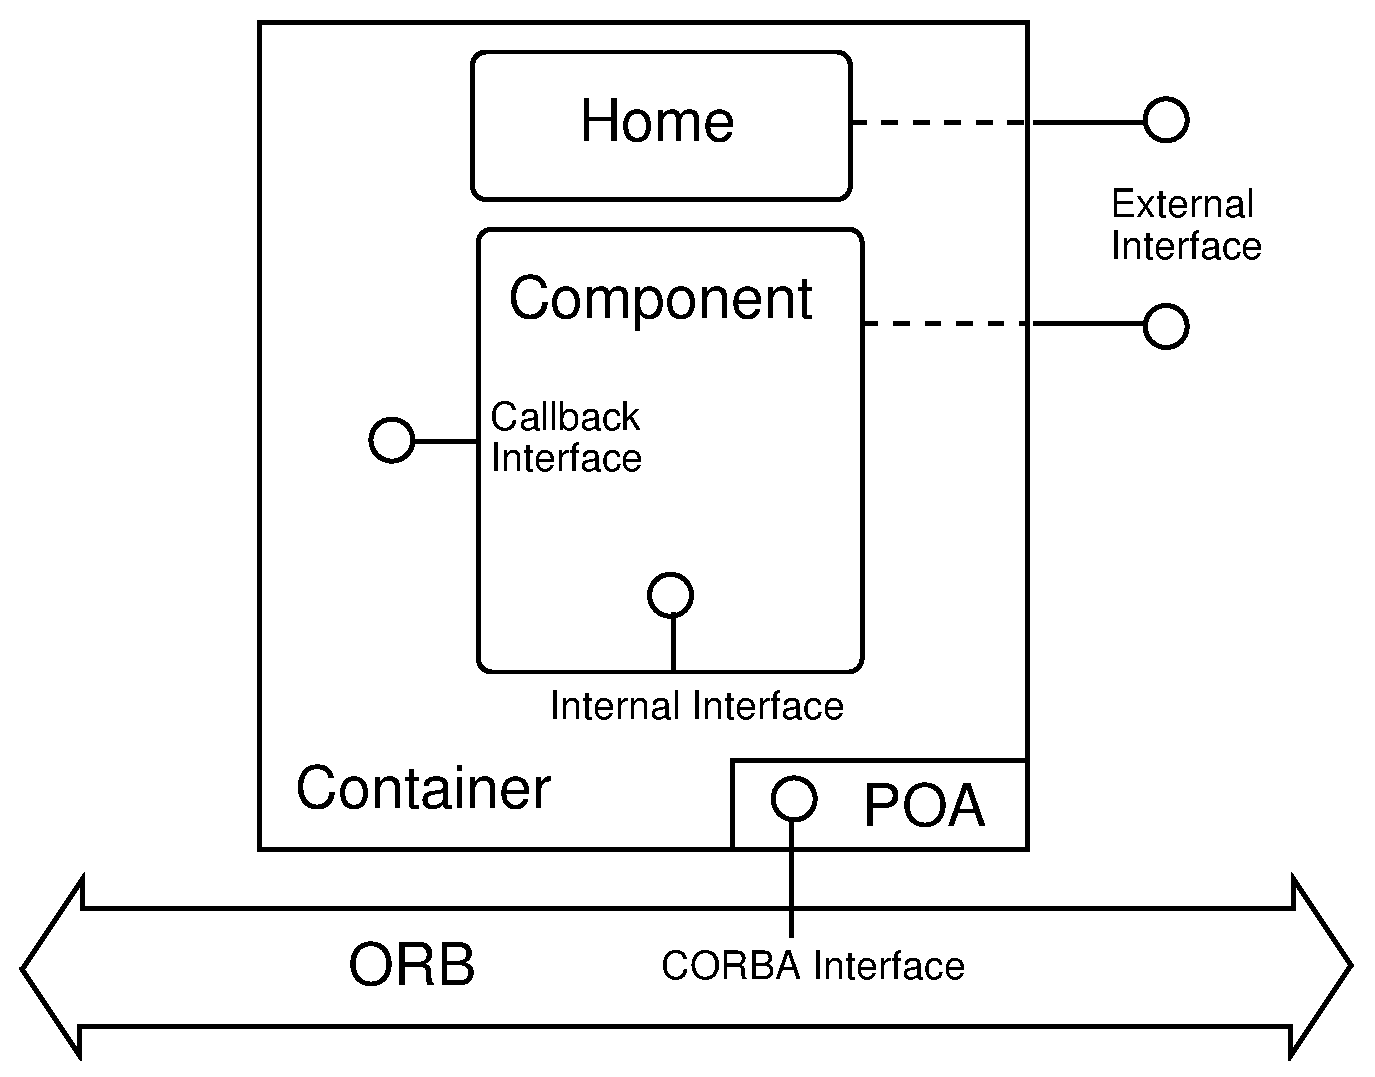
\includegraphics [width=6cm,angle=0] {Container}
        \caption{CCM container}
        \label{container}
    \end{center}
\end{figure}

As shown in Fig.~\ref{container}, the container programming model is made of the
following interfaces that are used by the client, the container and the
components:
\begin{description}
\item [Internal interfaces]
These local interfaces are used by the component developer and provided by the
container to assist in the implementation of the component's behavior.

\item [External interfaces] The external interfaces define the external view of
a component. They are used by the client and implemented by the component
developer.

\item [Callback interfaces]
These local interfaces are used by the container and implemented by the
component, either in generated code or directly, in order for the component to
be deployed in the container.
\end{description}

The CCM specification defined component categories whose behavior is specified
by the two container API types. Additionally there is a component category that
describe the empty container.
\begin{description}
\item [Service component]
The service component has behavior, no state and no identity. The lifespan of a
service component is equivalent to the lifetime of a single operation request.

\item [Session component]
The session component has behavior, transient state and a identity that is not
persistent. Note that the session component is equivalent to the stateful
session bean found in EJB.

\item [Process component]
The process component has behavior, persistent state which is not visible to the
client, and a persistent identity.

\item [Entity component]
The entity component has behavior, persistent state which is visible to the
client, and a identity which is visible to the clients through a primary key
declaration.

\end{description}



%==============================================================================
\section{Component assembly}
%==============================================================================

Connecting components by their ports leads to component {\it Assemblies} as
shown in Fig.~\ref{assemblygraph}.

\begin{figure}[htbp]
    \begin{center}
        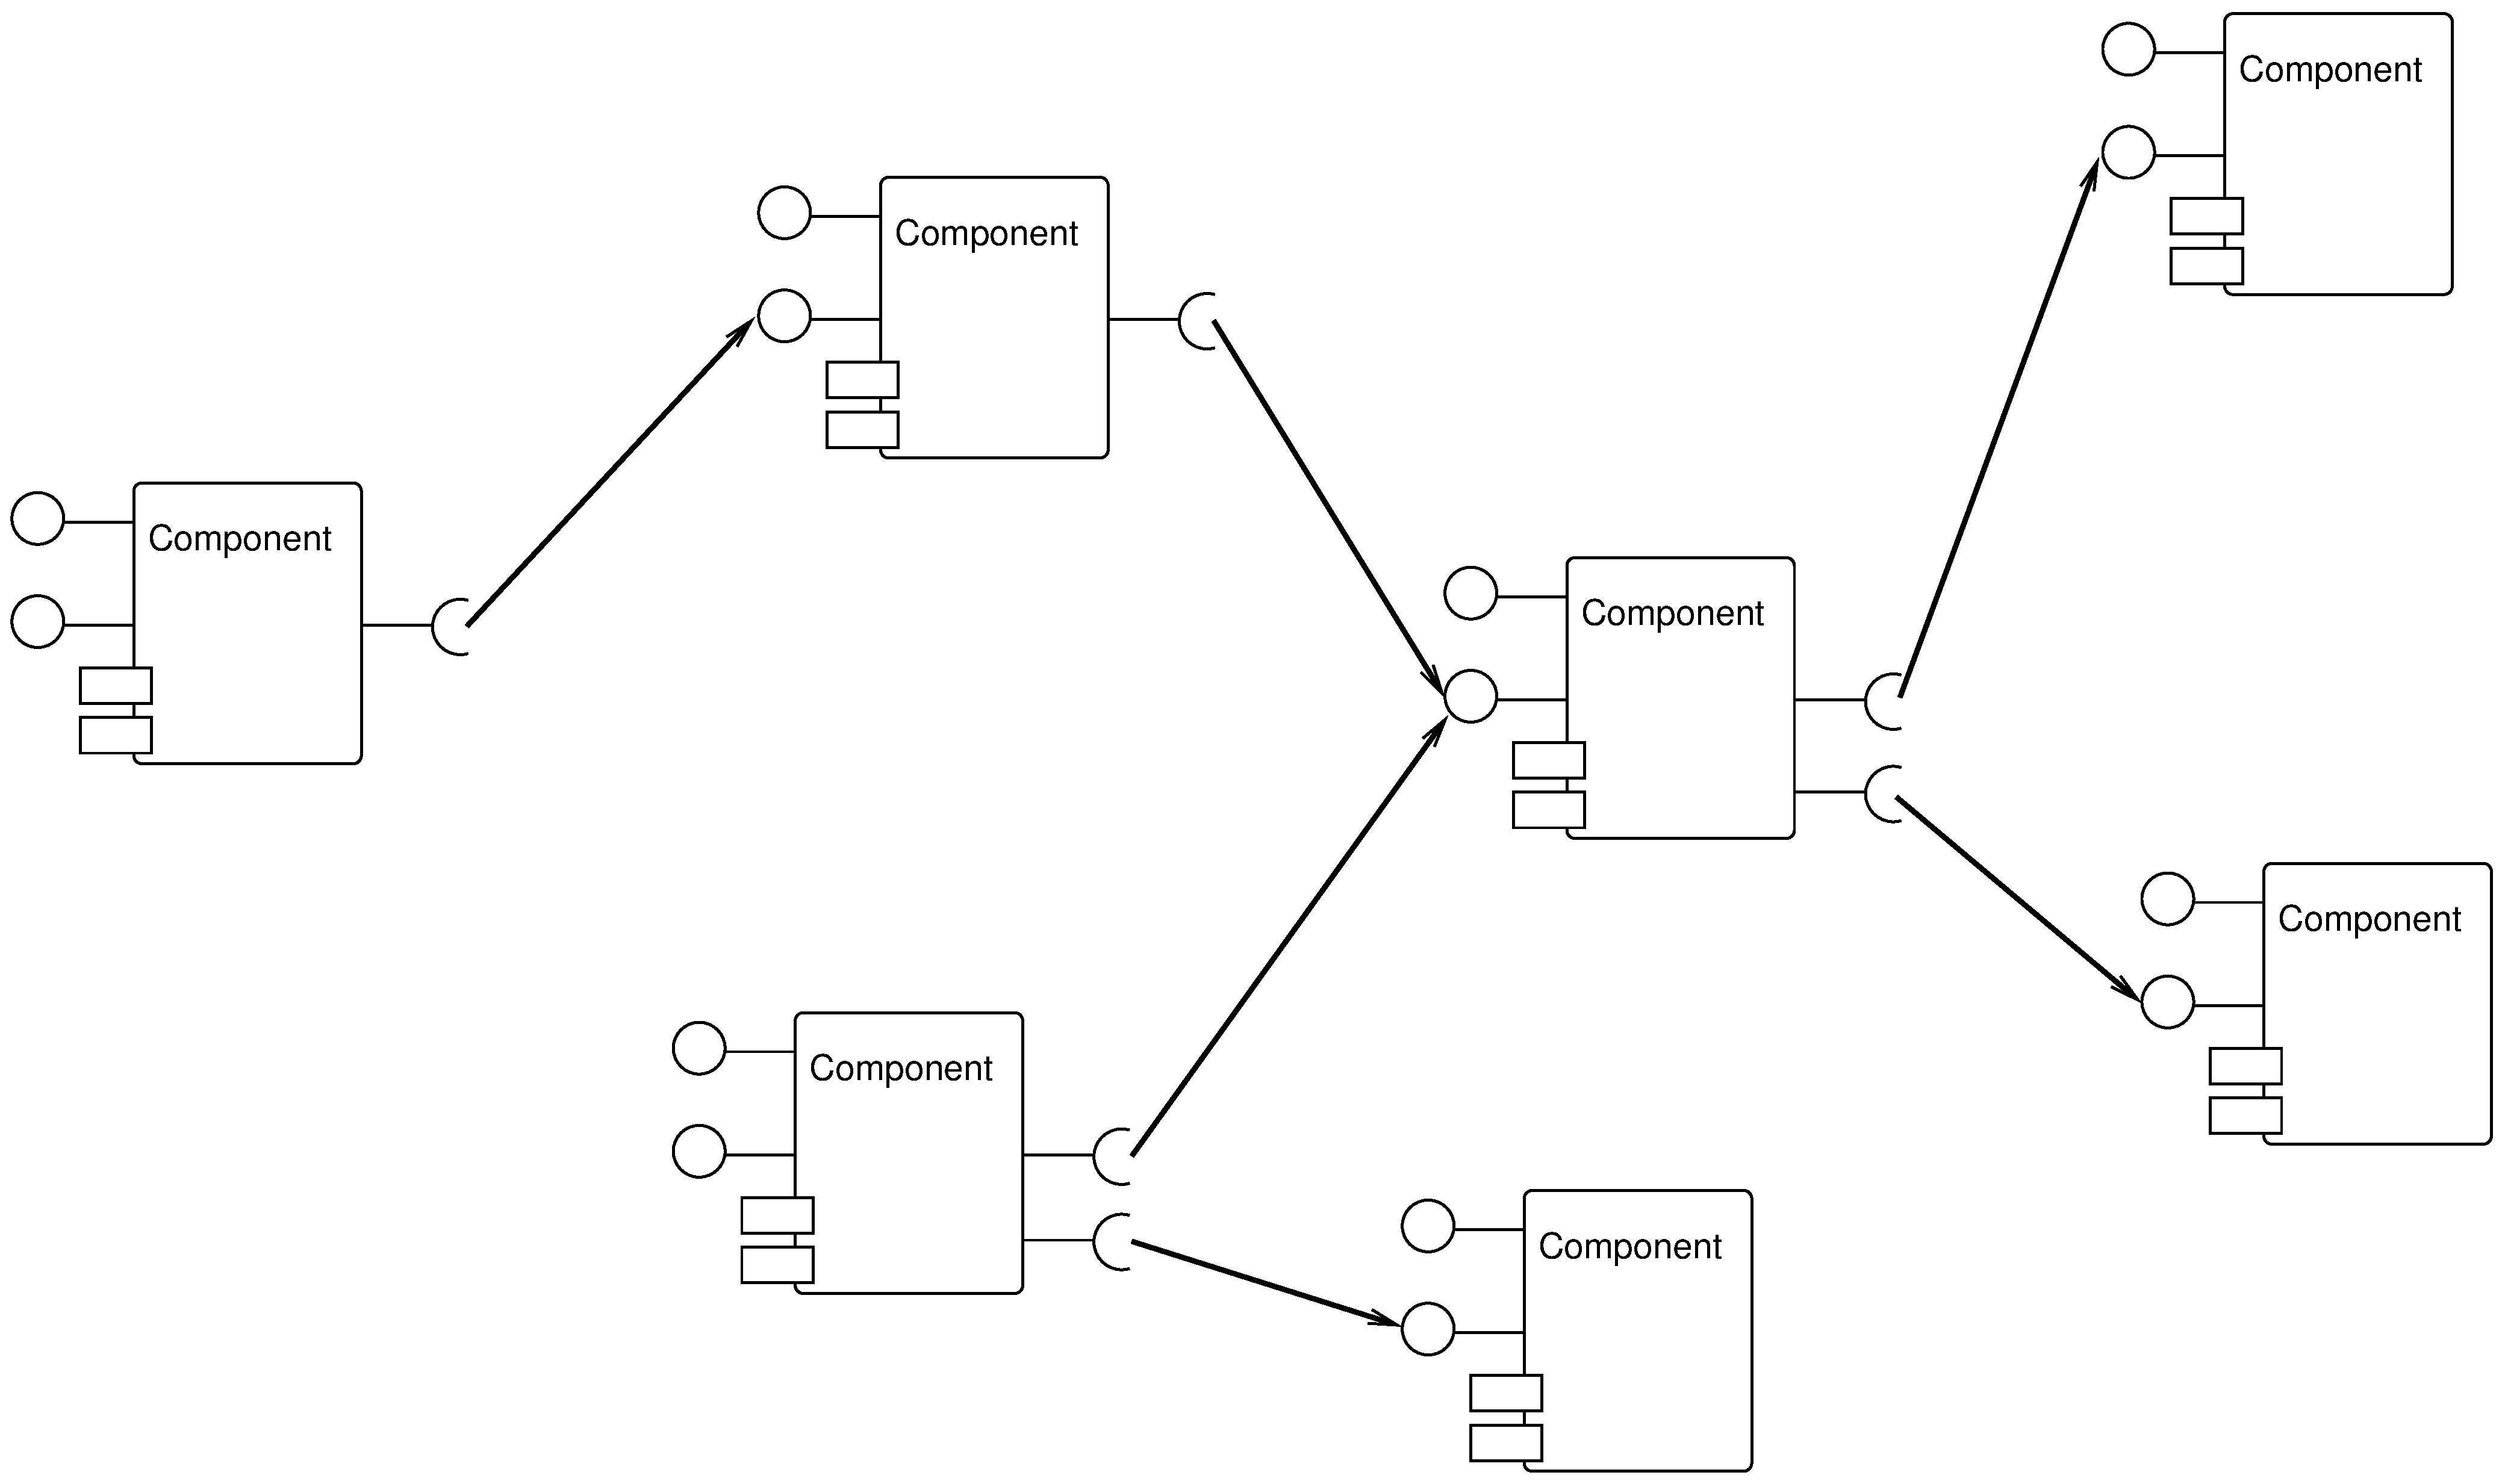
\includegraphics [width=6cm,angle=0] {Assembly}
        \caption{Component assembly}
        \label{assemblygraph}
    \end{center}
\end{figure}

The CCM specification defines an {\tt Components::Assembly} interface that
represents an assembly instantion. It is used to build up and tear down
component assemblies. Building the assembly up means creating all of the
components and establish connections between them as specified in the assembly
descriptor. Tearing the assembly down means removing all connections and
destroying the components.


%==============================================================================
\section{Descriptor files}
%==============================================================================

The CCM specification defines a bunch of XML descriptor files that are used to
describe software packages, components, properties and assemblies.
\begin{description}
\item [Software package descriptor (*.csd)]
The software package descriptor consists of general information about the
software followed by one or more sections describing implementations of
software.

\item [CORBA component descriptor (*.ccd)]
The component descriptor specifies component characteristics that a design tool
my use to display information about a component (e.g. supported interfaces,
inherited components, used and provided ports, etc.).

\item [Component assembly descriptor (*.cad)]
The assembly descriptor consists of elements describing the components used in
the assembly, connection information and partitioning information.

\item [Property file descriptor (*.cpf)]
The property file is used at deployment time to configure a home or a component
instance. A configurator uses the property file to determine how to set
component and home property attributes.
\end{description}


%==============================================================================
\section{Client programming model}
%==============================================================================

The client interacts with a CORBA component through two forms of external
interfaces, a home interface and one or more application interfaces. Two forms
of clients are supported by the CCM specification:
\begin{description}
\item [Component--aware client] 
This client knows that it is making requests against a component. The client can
use component mechanisms like navigation between component and facets etc.
Component--aware clients locates their interfaces using the {\tt
Components::HomeFinder} or a naming service.

A reference that supports the {\tt HomeFinder} interface may be obtained from
the ORB by invoking {\tt CORBA::ORB::resolve\_initial\_references()} with the
parameter value {\tt ``ComponentHomeFinder''}.

\item [Component--unaware client]
This client does not know that there is a CORBA component, the client requests
to ordinary CORBA objects and object factories.
\end{description}




%==============================================================================
\chapter{Local CCM Components}
%==============================================================================

From practical experiences we have learned that there is a need for improvements in
CCM to be usable. The following sections describe the new concepts 
\cite{TMKKW-EUROMICRO:2002,TKKKW-MIDDLEWARE:2003}
we introduced in respect to the CCM specification.


%==============================================================================
\section{Remote components}
%==============================================================================

The CCM specification describes only remote components where all ports are
accessible from CORBA clients. Some open source implementations like MicoCCM
\cite{MicoCCM} and OpenCCM \cite{MarvieMerle2001} implement this type of
components.

In such implementations, each remote component is accessible from any point in
the network, but communication between components in the same address space is
very expensive because method calls still have to go through the CORBA Object
Request Broker (ORB).

There are some techniques for transparently optimizing communication overhead
(e.g. CORBA collocation \cite{ObjectInterconnections18, wang00optimizing}), but
compared to pure local method invocations, a noticeable overhead still remains. 


%==============================================================================
\section{Local components}
%==============================================================================

To implement thin components in the same address space we need a specific
component model that defines local components and their interconnections. In
Java already exists such a thin component model (JavaBeans
\cite{Englander1997}), but in other languages like C++ and Python there are no
such specifications.

There is a need for a language independent local component model with
mappings to many different programming languages. Instead of inventing another
new component model, we use the CORBA Component Model in a local manner.


%==============================================================================
\section{Local component adapters}
%==============================================================================

The CCM specification hides most of the CORBA programming details from the
application developer, but it still forces developers to deal with CORBA
references, data types and memory management. While the OMG Java mapping
\cite{OMGIDL2Java} is acceptable in this regard, the C++ mapping
\cite{OMGIDL2Cpp} does not use advantages of standard C++ like strings,
vectors and lists.

To improve the usability of CCM, we proposed a new approach
that provides an easy way to implement components without having to pay 
attention to CORBA details.
We implement all business logic in local components without CORBA.
As shown in Fig.~\ref{LcacOverview}, these local components can be embedded
in a regular CORBA component using a set of adapters $A$.

\begin{figure}[!htb]
    \begin{center}
        \includegraphics [width=7cm,angle=0] {figures/LCAC_Overview}
        \caption{Local component adapter}
        \label{LcacOverview}
    \end{center}
\end{figure}

For every IDL interface or component, we generate corresponding interfaces in the
native implementation language. Adapter classes \cite{Gamma95} provide the
CORBA mapping, and link the business logic to a corresponding CORBA component.

As shown in Fig.~\ref{LcacLayerModel}, there is a local path and a remote path
between two component implementations. When running components in the same
address space, there is no need for CORBA communication. Using the local path
for connecting components significantly reduces the communication overhead.

\begin{figure}[!htb]
    \begin{center}
        \includegraphics [width=8cm,angle=0] {figures/Adapter1}
        \caption{Local vs. remote connection}
        \label{LcacLayerModel}
    \end{center}
\end{figure}

It's important to keep in mind that these adapters do not change the client's
view of a component, so our approach still conforms to the CCM standard.



%==============================================================================
\section{Assemblies of local and remote components}
%==============================================================================

An important issues in {\it Component--Based Software Engineering}
(CBSE) \cite{Szyperski02,IVICA2002,CBSE2001,HerzumSims99} is component granularity. 
Fat components increase runtime performance, but their reuse is limited. 
On the other hand, thin components lead to significant communication overhead 
but are easy to reuse.

Enterprise JavaBeans (EJB), for example, also have a local component concept 
\cite{EJBSpecificationV2_1}: 
A whole bean can be declared as local or
remote by extending the {\tt EJBHome, EJBObject} interfaces or the 
{\tt EJBLocalHome, EJBLocalObject} interfaces respectively.

As with local EJBs, we use local components for thin components located in
the same address space to improve performance and reusability. In contrast to
local EJBs, however, we do not have to decide between a local or remote
component because we always implement a local one. After writing the business
logic we can leave some ports local while some other ports are made remotely
accessible by adding a remote adapter. 

Note that the decision between using the
local or remote adapters does not affect the implementation of the business
logic; in other words we can scale the remote accessibility of a component port
by port at deployment time.
With this approach, we can use the same component model for a wide range of
component implementations and programming languages.


A component assembly can be described as a directed graph where the nodes are component
instances and the edges are receptacle to facet connections.
We can build assemblies of local and remote components using the {\it Session Facade} 
pattern \cite{Marinescu02}.

\begin{figure}[!htb]
    \begin{center}
        \includegraphics [width=8cm,angle=0] {figures/AssemblyGraph}
         \caption{Assembly instance graphs}
        \label{instanceGraph}
    \end{center}
\end{figure}

If an instance of a remote session facade component is created, all connected local 
components also have to be instantiated and connected (Fig.~\ref{instanceGraph}). 

In other words, a {\tt create()} call to a remote session facade component's home 
creates an assembly instance where related components are instantiated and connected 
as described in the assembly descriptor. 
A CORBA reference to the assembly instance is returned by the {\tt create()} 
call to the client.

From the client's point of view, a session facade component is a fat remote
component. In fact, this fat component is an assembly instance graph consisting of
a remote session facade and local component instances that ensure easy reuse of 
business code.


\end{appendix}

%=References===================================================================
\bibliographystyle{plain}
\bibliography{cbse,doc,wx,pattern,se}

\end{document}

